\documentclass[12pt]{article} 
\usepackage{longtable}
\usepackage{makecell}
\usepackage{float}
\usepackage{graphicx}
\usepackage{bm}
\usepackage{placeins}
\usepackage{booktabs}
\usepackage{gensymb}
\usepackage{amssymb}
\usepackage{indentfirst}
\usepackage{threeparttable} 
\usepackage{multirow}
\usepackage{tabularx}
\usepackage{aligned-overset}
\usepackage[slantfont,boldfont]{xeCJK}
\usepackage{fontspec}
\renewcommand{\arraystretch}{1.5}
% \usepackage[paperwidth=21cm,paperheight=29.7cm]{geometry}
\usepackage[a4paper,margin=2cm]{geometry}
\setCJKmainfont{SimSun}
\setmainfont{SimSun}
\setsansfont{SimSun}
% 设置正文字体为四号（12pt）
% \renewcommand{\CJKmainfont}{SimSun}
\renewcommand{\CJKfamilydefault}{\CJKrmdefault}
\renewcommand{\normalsize}{\fontsize{12pt}{18pt}\selectfont}
\normalsize

\title{多普勒实验报告}
\author{2411545 邱凯锐}
\date{2025.10.24}

\begin{document}
\maketitle
\section{实验目的}

1.验证多普勒效应：测量超声接收器运动速度与接收频率之间的关系，验证多普勒效应，并由
f-V 关系直线的斜率求声速。 

2.多普勒效应的应用：利用多普勒效应测量物体运动过程中多个时间点的速度，查看V-t关系
曲线，或调阅有关测量数据，即可得出物体在运动过程中的速度变化情况，可研究： 

1) 自由落体运动，并由V-t关系直线的斜率求重力加速度。 

2) 简谐振动，可测量简谐振动的周期等参数，并与理论值比较。 

3) 匀加速直线运动，测量力、质量与加速度之间的关系，验证牛顿第二定律。 

4) 其它变速直线运动。 

3.自组实验：熟悉智能手机的传感器测量功能及相关软件Phyphox， 提高设计实验的能力。 

\section{实验原理}
\subsection{超声的多普勒效应}
\begin{figure}[H]
    \centering
    
\includegraphics[width=0.8\textwidth]{fig1.png}
    \caption{超声的多普勒效应示意图}
\end{figure}

根据声波的多普勒效应公式，当声源与接收器之间有相对运动时，接收器接收到的频率 $f$ 为：
\begin{equation}
    f=f_0\cdot\frac{u+V_1\cos\alpha_1}{u-V_2\cos\alpha_2}
\end{equation} 

式中 $f_0$ 为声源发射频率， $u$ 为声速， $V_1$ 为接收器运动速率， $\alpha_1$ 为声源与接收器连线与接收器运动
方向之间的夹角， $V_2$ 为声源运动速率， $\alpha_2$ 为声源与接收器连线与声源运动方向之间的夹角（如 Figure 1）。

若声源保持不动，运动物体上的接收器沿声源与接收器连线方向以速度 $V$ 运动，则从（1）式可
得接收器接收到的频率应为：
\begin{equation}
    f=f_0\cdot\left(1+\frac Vu \right)
\end{equation} 

当接收器向着声源运动时， $V$ 取正，反之取负。

若 $f_0$ 保持不变，以光电门测量物体的运动速度，并由仪器对接收器接收到的频率自动计数，根据
（2）式，作 $f-V$ 关系图可直观验证多普勒效应，且由实验点作直线，其斜率应为 $k=f_0/u$ ，由此可计
算出声速 $u=f_0/k$ 。 

由（2）式可解出：
\begin{equation}
    V=u\cdot\left(\frac f{f_0}-1 \right)
\end{equation}

若已知声速 $u$ 及声源频率 $f_0$ ，通过设置使仪器以某种时间间隔对接收器接收到的频率 $f$ 采样计数，
由微处理器按（3）式计算出接收器运动速度，由显示屏显示 $V-t$ 关系图，或调阅有关测量数据，即
可得出物体在运动过程中的速度变化情况，进而对物体运动状况及规律进行研究。 

\subsection{超声的红外调制与接收}
早期产品中，接收器接收的超声信号由导线接入实验仪进行处理。由于超声接收器安装在运动体
上，导线的存在对运动状态有一定影响，导线的折断也给使用带来麻烦。新仪器对接收到的超声信号
采用了无线的红外调制-发射-接收方式。即用超声接收器信号对红外波进行调制后发射，固定在运动
导轨一端的红外接收端接收红外信号后，再将超声信号解调出来。由于红外发射/接收的过程中信号
的传输是光速，远远大于声速，它引起的多普勒效应可忽略不计。采用此技术将实验中运动部分的导
线去掉，使得测量更准确，操作更方便。信号的调制-发射-接收-解调，在信号的无线传输过程中是一
种常用的技术。

\section{实验仪器}
多普勒效应综合实验仪由实验仪，超声发射/接收器，红外发射/接收器，导轨，运动小车，支架，
光电门，电磁铁，弹簧，滑轮，砝码及电机控制器等组成。实验仪内置微处理器，带有液晶显示屏，
Figure 2 为实验仪的面板图。 

\begin{figure}[H]
    \centering
    
\includegraphics[width=0.6\textwidth]{fig2.png}
    \caption{多普勒实验仪面板图}
\end{figure}

\section{实验内容}

\subsection{验证多普勒效应并由测量数据计算声速}
让小车以不同速度通过光电门，仪器自动记录小车通过光电门时的平均运动速度及与之对应的平
均接收频率。由仪器显示的 $f-V$ 关系图可看出速度与频率的关系，若测量点成直线，符合（2）式描
述的规律，即直观验证了多普勒效应。用作图法或线性回归法计算 $f-V$ 直线的斜率 $k$ ，由 $k$ 计算声速
$u$ 并与声速的理论值比较，计算其百分误差。

\subsubsection{仪器安装}
如 Figure 3 所示。所有需固定的附件均安装在导轨上，将小车置于导轨上，使其能沿导轨自由滑动，
此时，水平超声发射器、超声接收器组件（已固定在小车上）、红外接收器在同一轴线上。将组件电
缆接入实验仪的对应接口上。安装完毕后，电磁铁组件放在轨道旁边，通过连接线给小车上的传感器
充电，第一次充电时间约6～8秒，充满后(仪器面板充电灯变黄色或红色)可以持续使用4～5分钟。
充电完成后连接线从小车上取下，以免影响小车运动。 

\begin{figure}[H]
    \centering
    
\includegraphics[width=0.8\textwidth]{fig3.png}
    \caption{实验装置示意图}
\end{figure}

\subsubsection{测量准备}
（1）实验前须要在每个速度下测试传送带松紧度是否合适，

（2）测试仪开机后，首先要求输入室温。因为计算物体运动速度时要代入声速，而声速是温度的
函数。将室温 $t_c$ 值调到实际值，按“确认”。 然后仪器将进行自动检测调谐频
率 $f_0$，约几秒钟后将自动得到调谐频率，将此频率 $f_0$ 记录下来，按“确认”进行后面实验

\subsubsection{测量步骤}
1) 在液晶显示屏上，选中“多普勒效应验证实验”，并按“确认”； 

2) 利用修改测试总次数（选择范围 5$\sim$10，因为有5种可变速度，一般选5次），
选中“开始测试”，但不要按“确认”；

3) 用电机控制器上的“变速”按钮选定一个速度。准备好后，按“确认”，再按电机控制器上
的“启动”键，测试开始进行，仪器自动记录小车通过光电门时的平均运动速度及与之对应
的平均接收频率； 

4) 每一次测试完成，都有“存入”或“重测”的提示，可根据实际情况选择，“确认”后回到
测试状态，并显示测试总次数及已完成的测试次数； 

5) 按电机控制器上的“变速”按钮，重新选择速度，重复步骤3、4； 

6) 完成设定的测量次数后，仪器自动存储数据，并显示 $f-V$ 关系图及测量数据。

\subsubsection{数据记录与处理}

由 $f-V$ 关系图可看出，若测量点成直线，符合（2）式描述的规律，即直观验证了多普勒效应。
用作图法或线性回归法计算 $f-V$ 关系直线的斜率 $k$ 。公式（4）为线性回归法计算 $k$ 值的公式，其中测
量次数 $i＝5$ 。
\begin{equation}
    k=\frac{\bar{V_i}\times\bar{f_i}-\bar{V_i\times F_i}}{\bar{V_i}^2-\bar{V_i^2}}
\end{equation}

由 $k$ 计算声速 $u = f_0/k$ ，并与声速的理论值比较，声速理论值由 $u_0 = 331(1＋t_c/273)^{1/2}$ 计算，
 $t_c$ 表示室温（摄氏温度，单位$^\circ \mathrm{C}$）。测量数据的记录是仪器自动进行的。在测量完成后，只需在出现
的显示界面上，翻阅数据并记入 Table 1 中，然后按照上述公式计算出相关结果并填入表格。 

\begin{figure}[H]
    \centering
    
\includegraphics[width=0.8\textwidth]{fig4.png}
    \caption{$f-V$ 关系图}
\end{figure}

\begin{table}[H]
    \centering
    \caption{多普勒效应的验证与声速的测量}
    \vspace{2pt}
    \begin{minipage}{0.7\textwidth}
        \raggedleft
        $t_c=15 ~^\circ \mathrm C $ ，$f_0=40001 \mathrm{Hz}$
    \end{minipage}\\[2pt]
    \small
    % ↓↓↓ 缩放开始
    \resizebox{0.9\textwidth}{!}{%
    \begin{tabular}{|cccccc|c|c|c|c|}
    \hline
    \multicolumn{6}{|c|}{测量数据}                                                                                                                                              & \multirow{2}{*}{\begin{tabular}[c]{@{}c@{}}直线斜率\\ $k\ (\mathrm{m^{-1}})$\end{tabular}} & \multirow{2}{*}{\begin{tabular}[c]{@{}c@{}}声速测量值\\ $u=f_0/k (\mathrm {m/s})$\end{tabular}} & \multirow{2}{*}{\begin{tabular}[c]{@{}c@{}}声速理论值\\ $u_0(\mathrm{m/s})$\end{tabular}} & \multirow{2}{*}{\begin{tabular}[c]{@{}c@{}}百分误差\\ $(u-u_0)/u_0$\end{tabular}} \\ \cline{1-6}
    \multicolumn{1}{|c|}{次数 $i$}                & \multicolumn{1}{c|}{1}     & \multicolumn{1}{c|}{2}     & \multicolumn{1}{c|}{3}     & \multicolumn{1}{c|}{4}     & 5     &                                                                                        &                                                                                            &                                                                                      &                                                                               \\ \hline
    \multicolumn{1}{|c|}{$V_i\ (\mathrm{m/s})$} & \multicolumn{1}{c|}{0.9}   & \multicolumn{1}{c|}{0.39}  & \multicolumn{1}{c|}{0.75}  & \multicolumn{1}{c|}{0.65}  & 0.56  & \multirow{2}{*}{110.69}                                                                & \multirow{2}{*}{393.37}                                                                    & \multirow{2}{*}{339.97}                                                              & \multirow{2}{*}{15.71\%}                                                      \\ \cline{1-6}
    \multicolumn{1}{|c|}{$f_i\ (\mathrm{Hz})$}  & \multicolumn{1}{c|}{40105} & \multicolumn{1}{c|}{40054} & \multicolumn{1}{c|}{40088} & \multicolumn{1}{c|}{40077} & 40066 &                                                                                        &                                                                                            &                                                                                      &                                                                               \\ \hline
    \end{tabular}
    } % ← 缩放结束
\end{table}

\subsubsection{误差分析}
1） 小车传送带松紧调节不合适，导致小车速度并不稳定；

2）光电门没有调节至完全水平，且与小车发生些许触碰，导致速度测量偏小；

3）测量组数偏少，偶然误差影响较大；

4）超声波发射器、小车传感器和红外接收器未水平共轴，导致频率测量有误。

\subsection{水平谐振运动装置的测量}
按 Figure 5 安装水平谐振运动装置。设置采样数为 60，采样间隔为 80ms ，对用两根弹簧拉着的
小车（小车及支架上留有弹簧挂钩孔）所做水平阻尼振动的一次测量及显示实例。（在实验中，可以
将小车上传感器和电磁阀用充电电缆连接，保证实验连续）。

\begin{figure}[h]
    \centering
    
\includegraphics[width=0.6\textwidth]{fig5.png}
    \caption{水平谐振实验}
\end{figure}

\begin{figure}[H]
    \centering
    
\includegraphics[width=0.6\textwidth]{fig6.jpg}
    \caption{ $\bar v-t$  关系图}
\end{figure}

\begin{figure}[H]
    \centering
    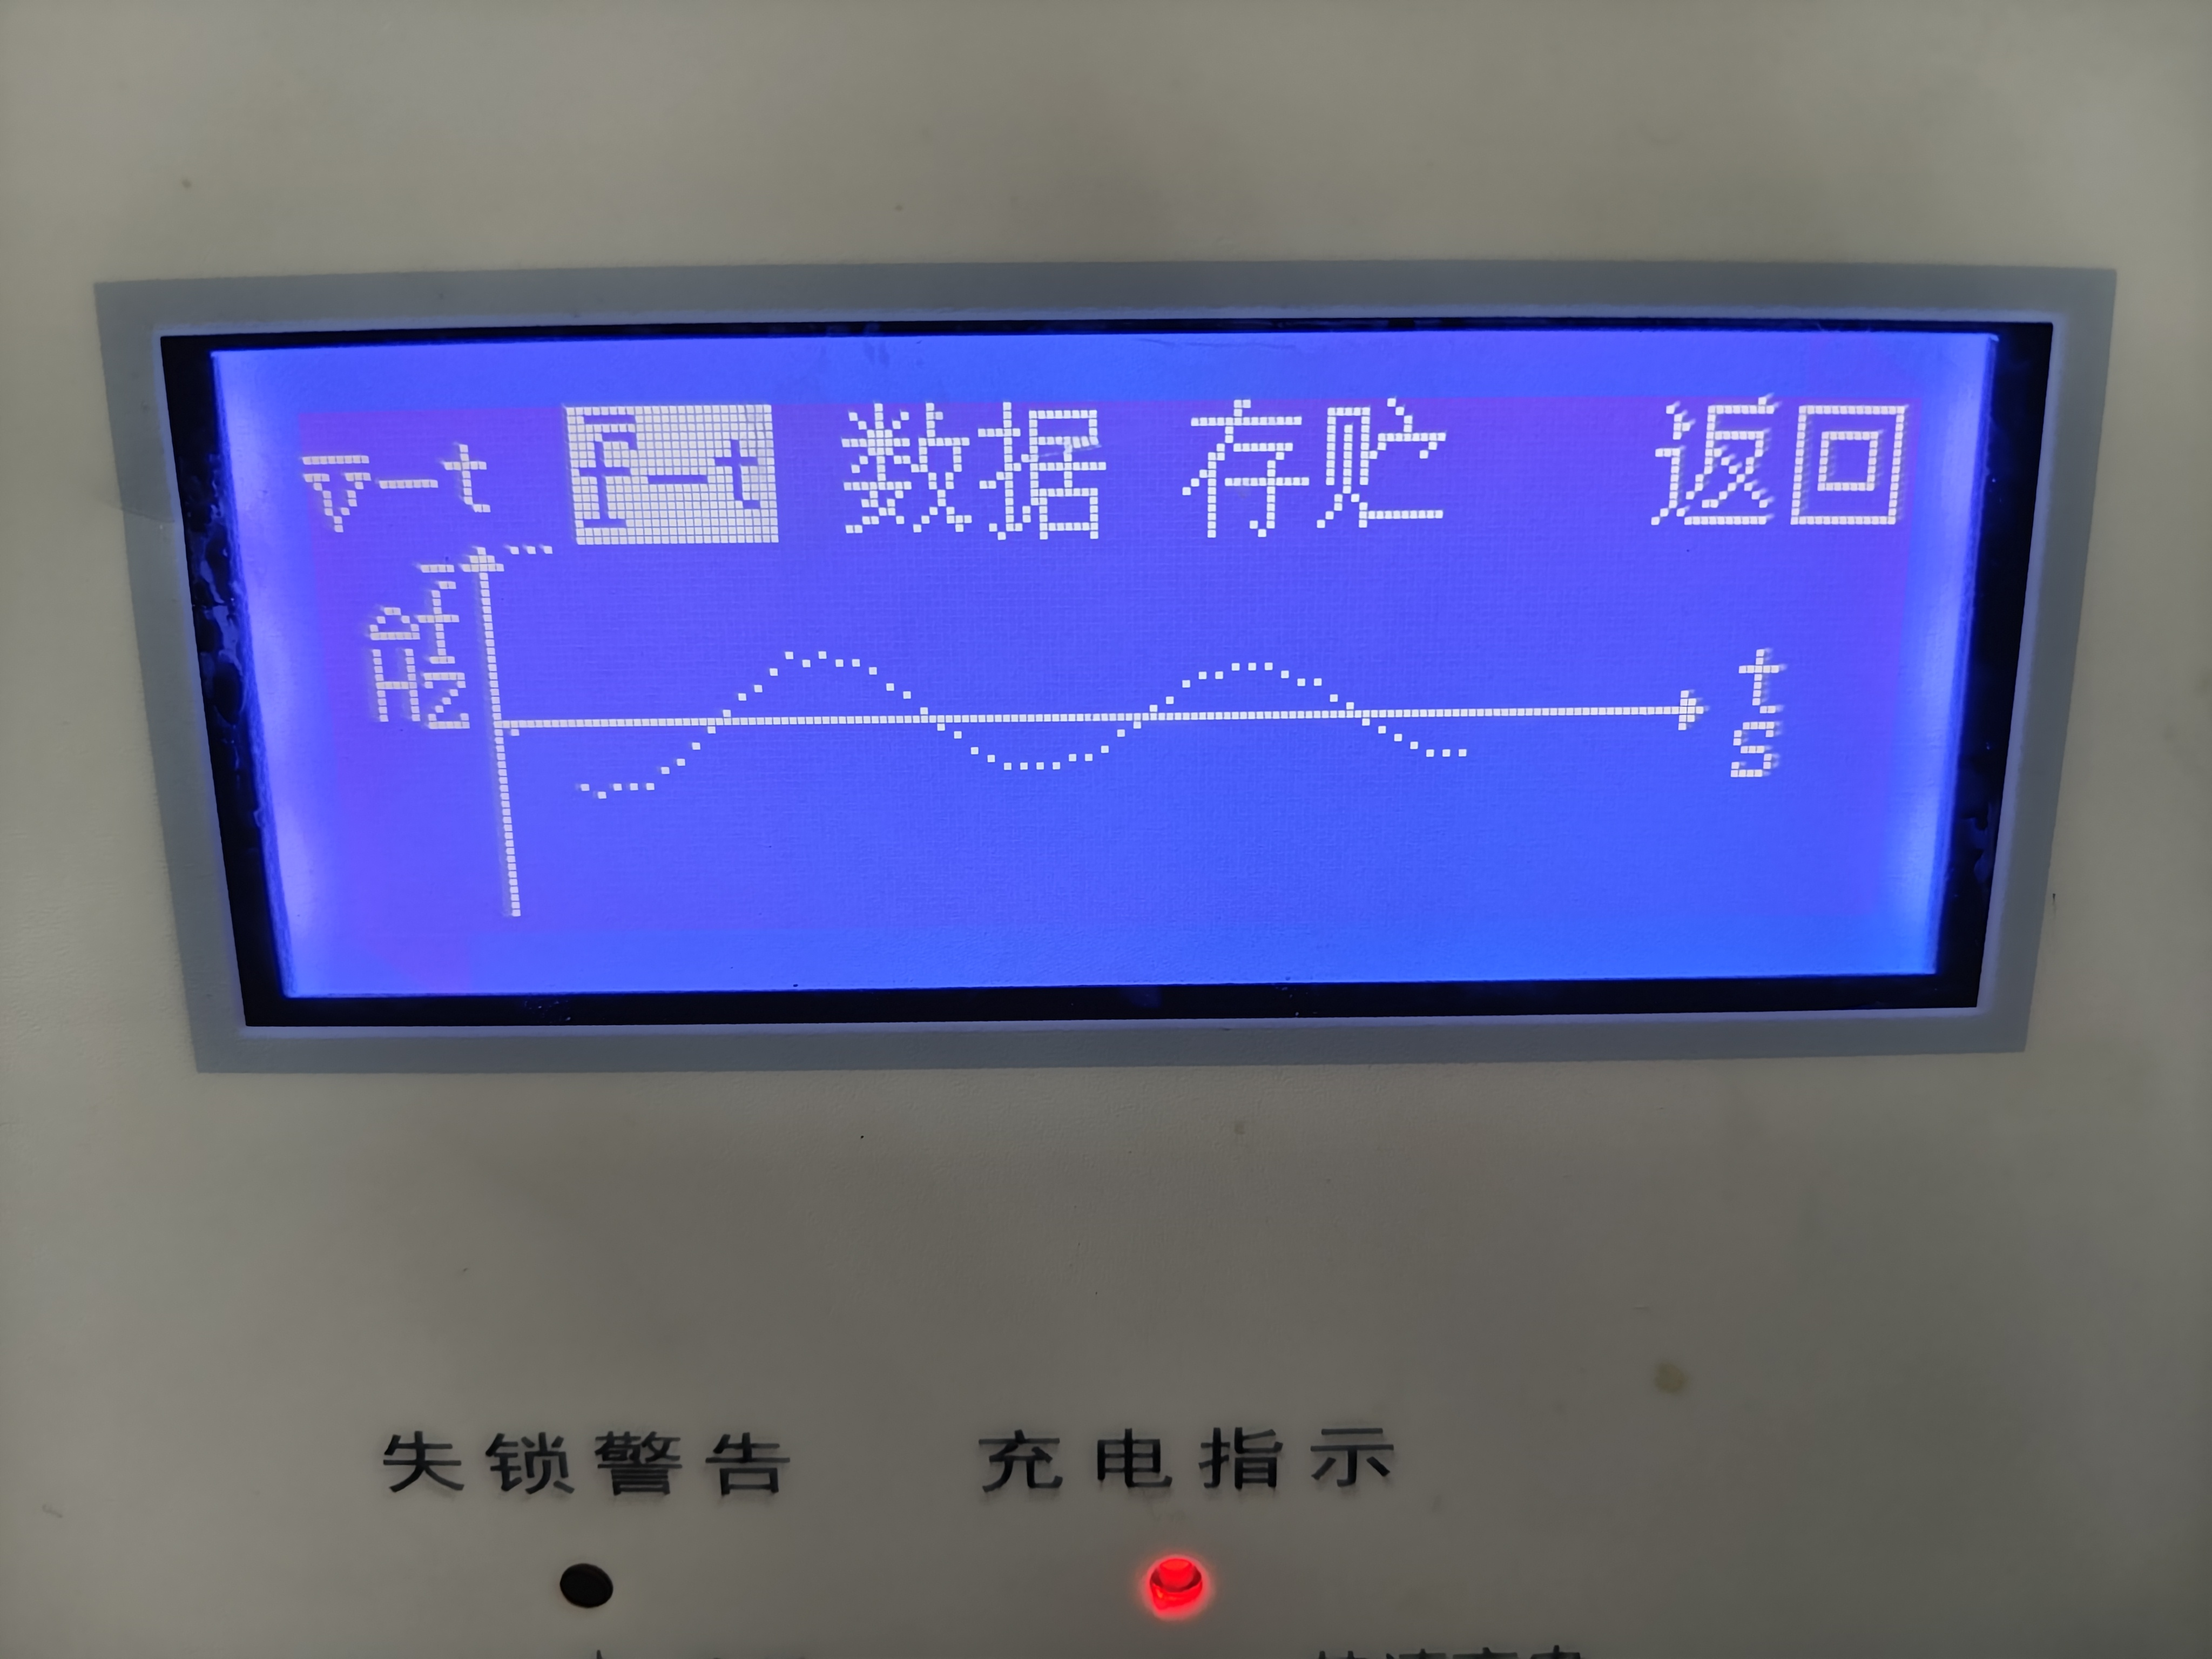
\includegraphics[width=0.6\textwidth]{fig7.jpg}
    \caption{ $\bar f-t$ 关系图}
\end{figure}

\subsection{设计性实验-研究单摆运动}
\subsubsection{实验内容}
用手机和细绳组合成一个单摆，改变摆长，利用手机软件测量单摆的运动周期。

\begin{table}[H]
    \centering
    \caption{多普勒效应的验证与声速的测量}
    \vspace{2pt}
    \begin{minipage}{0.7\textwidth}
        \raggedleft
        手机对角线长 $d=17.00cm$
    \end{minipage}\\[2pt]
    \small
    % ↓↓↓ 缩放开始
    % \resizebox{0.9\textwidth}{!}{%
    \begin{tabular}{|c|c|c|c|c|}
        \hline
        次数 $i$                & 1     & 2     & 3     & 4     \\ \hline
        摆长 $L_i(\mathrm{cm})$ & 29.20 & 40.70 & 52.00 & 68.40 \\ \hline
        周期 $T_i(\mathrm{s})$  & 1.19  & 1.32  & 1.58  & 1.76  \\ \hline
    \end{tabular}
    % } % ← 缩放结束
\end{table}

\begin{figure}[H]
    \centering
    \rotatebox{90}{% 旋转 90 度（顺时针），改成 -90 可反方向
        
\includegraphics[width=0.5\textwidth]{fig8.jpg}
    }
    \caption{手机单摆}
\end{figure}

\begin{figure}[H]
    \centering
    
\includegraphics[width=0.8\textwidth]{fig6.png}
    \caption{ $T^2-L$拟合曲线}
\end{figure}

根据单摆周期公式
\begin{equation}
    T^2=\frac{4\pi^2 L}{g}
\end{equation}
得到重力加速度 $g=8.811\ \mathrm {m\cdot s^{-2}}$，相对误差 $E=\frac{|g_0-g|}{g_0}=10.1\%$

误差分析：
\begin{itemize}
    \item 手机测量较为不稳定，误差较大；
    \item 手机在摆动过程中很容易发生自旋，使得周期测量不准确；
    \item 手机的摆动很大程度上并不是在一个竖直平面内；
    \item 单摆上端的固定不是牢固，导致摆长变化；
    \item 摆动的角度过大，和理想的单摆有区别。
\end{itemize}


\subsubsection{自拟思考题}
（1）\textbf{怎么减小手机在摆动过程中的自旋？}

可以改进手机释放的位置、角度和方法，尽可能减小手机的自旋。或者增加手机的悬挂点，减小转动的自由度。

（2）\textbf{分析以上数据实验结果，同实验室中其他方法研究单摆运动做比较。}

利用手机进行实验的实验结果，可以较为粗糙地研究单摆运动以及测量重力加速度。与其他方法相比，误差较大，但是优势在于，实验装置简单，操作快捷。

（3）\textbf{查阅资料，手机传感器是如何测量摆动周期的？}

手机加速度计（accelerometer）最常被用来测量单摆/摆动周期：摆动时机体相对于重力的投影随角度变化呈近似正弦波，加速度计在手机固定于摆锤上时能记录到这个周期性信号，然后通过峰值/零交叉/FFT等方法提取周期。
\end{document}